%_______________________________________________________________________________
% main.tex

\input{preamble12.tex}
\hypersetup{%
    pdfauthor={Mike Pierce}%
   ,pdftitle={Pop Quiz | Math 113}%
   ,pdfkeywords={Pierce,CMU,Colorado,College Algebra,113}%
   ,pageanchor=false%
}
\geometry{
    margin=1in%
   ,left=0.75in%
   ,right=0.75in%
}
\usepackage{fourier}
\usepackage[default]{comicneue}
\input{accessible-colors.tex}
\input{newcommand.tex}
\input{newenvironment.tex}
\pagenumbering{gobble}
\usepackage{pagegrid}
\pagegridsetup{
    step=0.5in
    ,firstcolor=blue
    ,secondcolor=orange
    ,foreground=true
    ,disable
}


\begin{document}

\begin{center}
    {\Huge{Pop Quiz}}
    \\ Math 113-001/6 College Algebra
    \\ Colorado Mesa University Fall 2022
\end{center}

\vspace{0.5in-2px}
%\vspace{2em}
%\textsc{Name}: \enspace \hrulefill
%\vspace{1em}

\begin{enumerate}

    \item 
        What are the coordinates of the vertex
        and of the two \(x\)-intercepts of the parabola
        that is the graph of \(f(x) = -\frac{7}{4}(x-3)^2+7 \)?
        \vfill\null
        \vfill\null

    \item 
        The function \(f\) defined by the formula
        \[f(x) = \frac{7}{x-1}+4\]
        is a one-to-one function.
        Write down a formula for its inverse function \(\inv{f}\).
        \vfill\null
        \vfill\null

    \item 
        If \(f(x) = 3x^2-5\) and \(g(x) = |x-9|\),
        what is a formula for \(f \compose g\)?
        What is a formula for \(g \compose f\)?
        \vfill\null

        \newpage

    \item 
        Below is the graph of a function \(f(x)\).
        \begin{figure}[h]
            \centering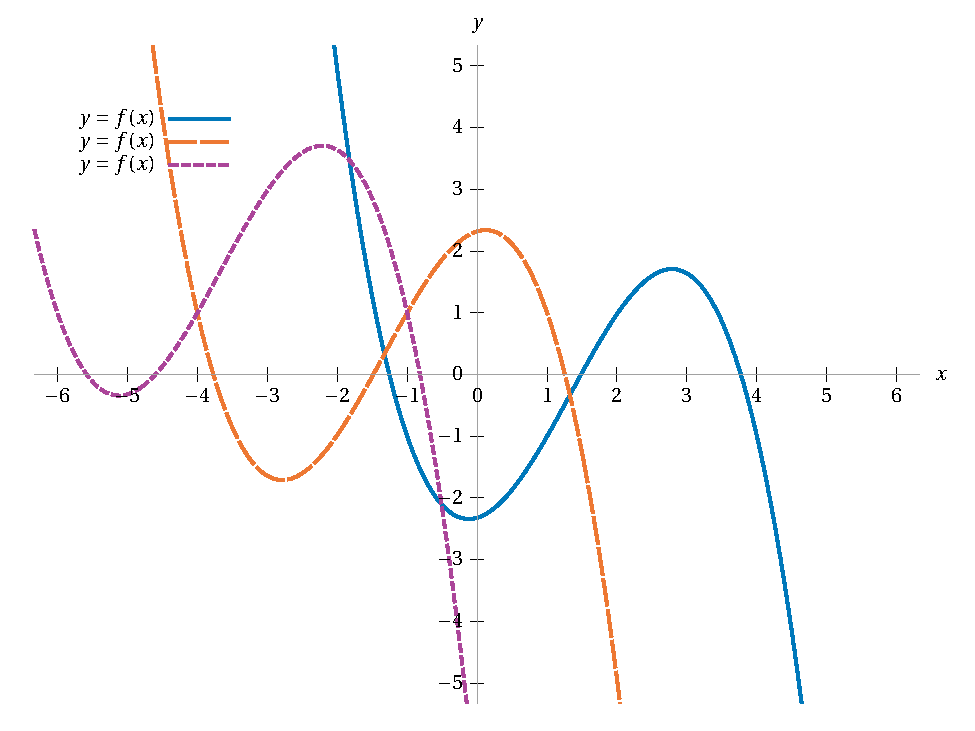
\includegraphics[width=\textwidth]{figures/transform/main.pdf}
        \end{figure}
        \begin{enumerate}
            \item 
                On this same set of axes, 
                sketch the graph of the function \(-f(-x)\).
                \vfill\null
            \item 
                On this same set of axes, 
                sketch the graph of the function \(f(x+5)+2\).
                \vfill\null
            \item 
                On this same set of axes, 
                sketch the graph of the function \(|f(x)|\).
                \vfill\null
        \end{enumerate}

\end{enumerate}

\end{document}

